%!TEX root = ../2019_7_Ozgumus_Semsi_Yigit.tex

\begingroup

\begingroup
{
	\color{Green}

This chapter presents the developments in the field of anomaly detection and generative adversarial
networks. Although the models introduced in Chapter \ref{chap:sota} deliver certain level of
performance, potential improvements are still a possibility. These improvements are related to both
adversarial training of the generator and discriminator networks and applying different training strategy to 
stabilize the training of encoder network presented in the overall model. Section \ref{sec:fanogan} and 
\ref{sec:ebgan} presents some of these improvements that are later adopted by our model. Their contribution
to solve the disadvantages we observed in the previous model will be discussed. 

\section{F-AnoGAN }
\label{sec:fanogan}

AnoGAN \cite{Schlegl2017UnsupervisedAD} is considered as the first moel that uses generative
adversarial networks for an anomaly detection task. The main problems with this model, are the
stabilization issues of the adversarial training, and inference stage of the model that
maps from the latent representation to the input data distribution
as the inverse mapping of generator network. Model used back propagation to approximate the latent
representation for every query image to compute the anomaly score which resulted a very poor
performance in terms of the computation time. This was the main disadvantage of the model
because it is very challenging to integrate into a real life application with an implausible
inference time. F-AnoGAN (Fast AnoGAN ) model \cite{pub.1111824956} aims to eliminate the inference computation time 
problem by implementing an encoder network with a new training strategy. It also uses a new objective function for the adversarial
training to further stabilize the generator discriminator performance. In the rest of this section,
F-AnoGAN model, its training strategies and anomaly detection methods will be discussed.

Architecture of F-AnoGAN is very similar to the BiGAN \cite{Donahue2017AdversarialFL}
model. It consists of a generator discriminator for the adversarial learning and an encoder
network to learn the inverse mapping from latent representation to the input image data.
\begin{figure}[h!]
	\centering
	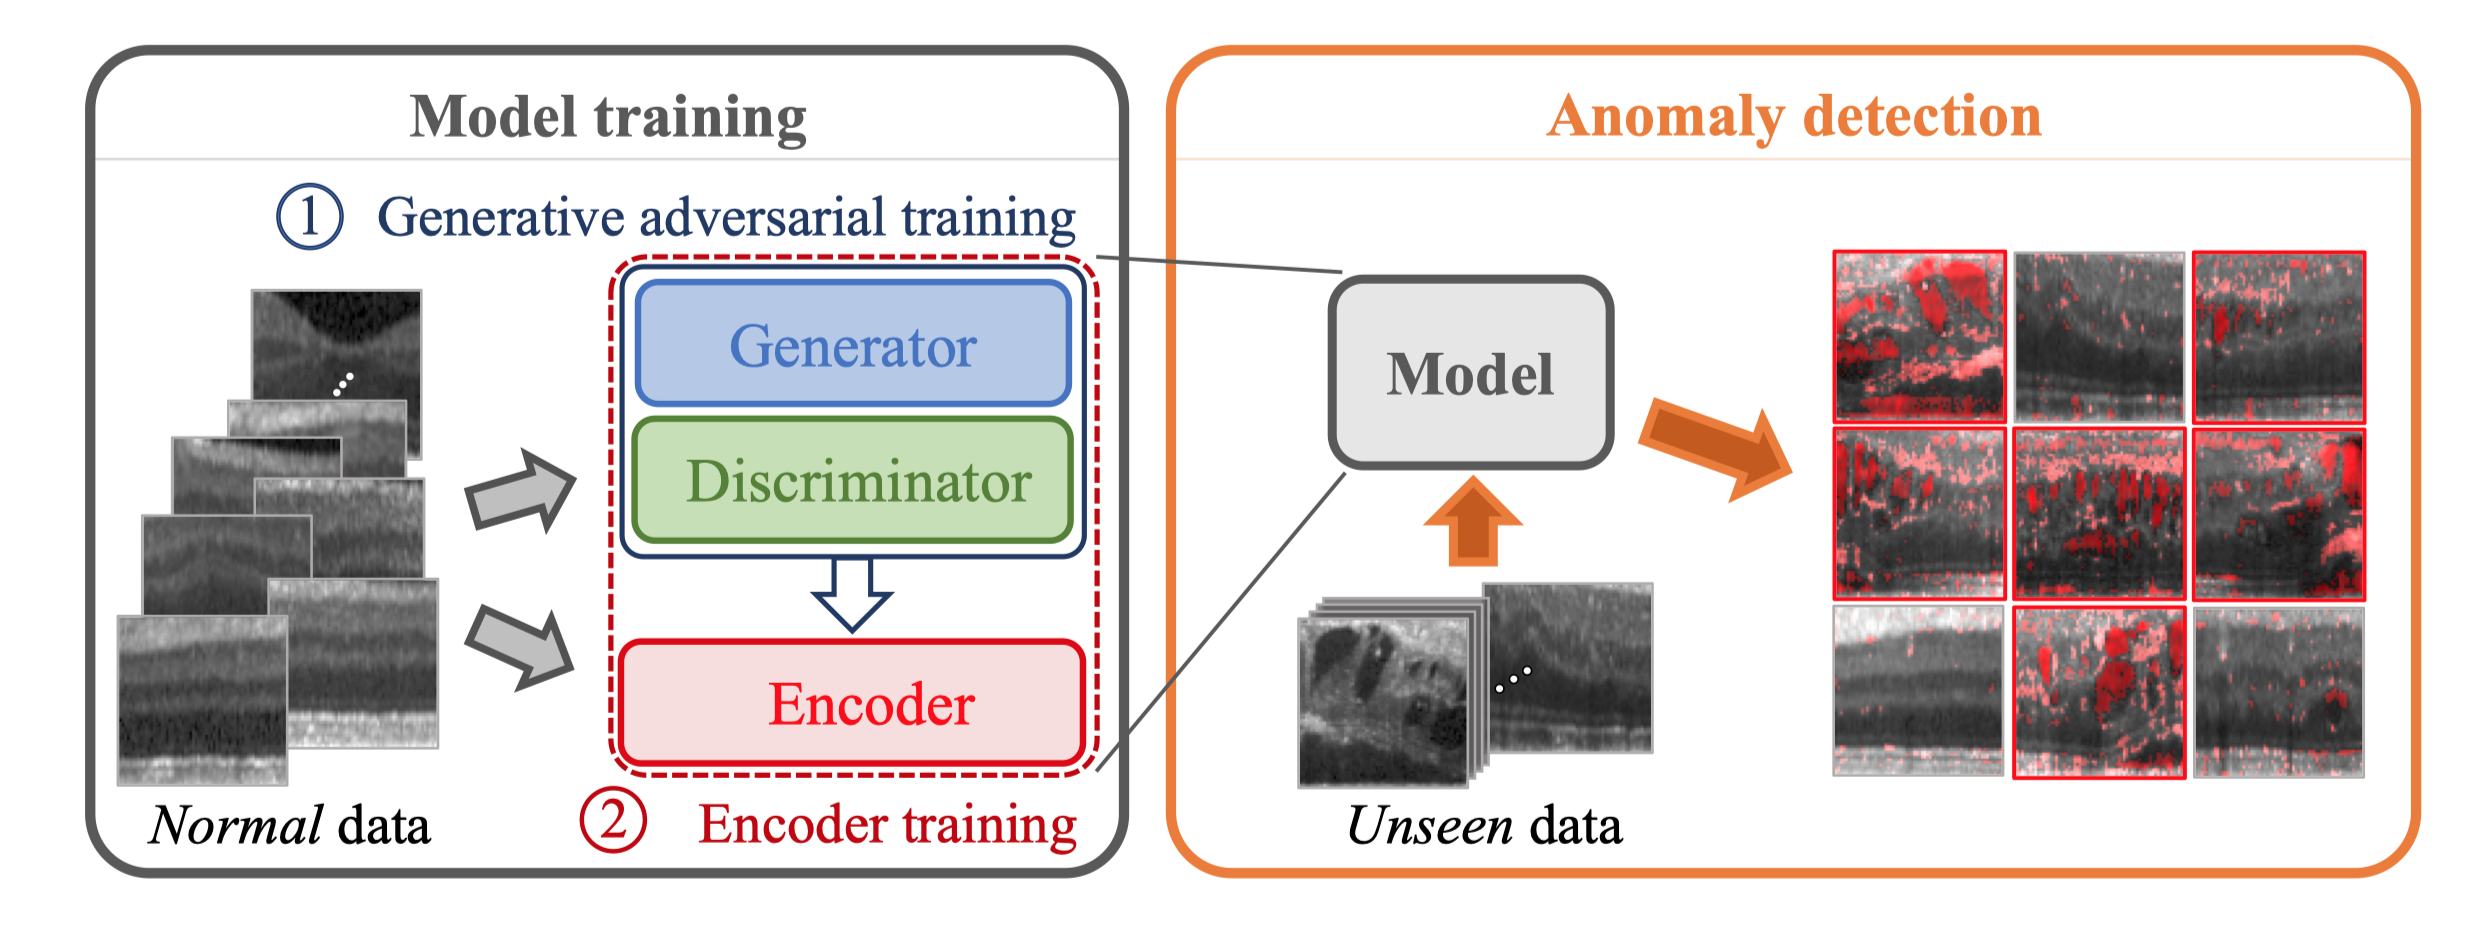
\includegraphics[width=.9\textwidth]{fanogan_framework}
	\caption{F-AnoGAN Model Overview \cite{pub.1111824956}}
	\label{fig:fanogan_network}
\end{figure}

The first improvement is the change of training style of the whole model. In BiGAN approach,
encoder and generator networks are trained simultaneously to fool the discriminator. Hence discriminator is
modified to classify the pairs of noise (latent representation) and images instead of the single
image approach used in the GAN. It tries to distinguish samples from a joint
distribution which explained in Section \ref{sec:bigan}. Including encoder to the adversarial setup
also introduces instability issues which ALAD model \cite{DBLP:journals/corr/abs-1812-02288}
tried to mitigate with additional discriminators that approximate conditional entropy. (see Section
\ref{sec:alad_alice}). F-AnoGAN model addresses this issue by separating the training of
encoder network $E$ from the generator discriminator networks. New model can be seen in Figure
\ref{fig:fanogan_training}. 
\begin{figure}[h!]
	\centering
	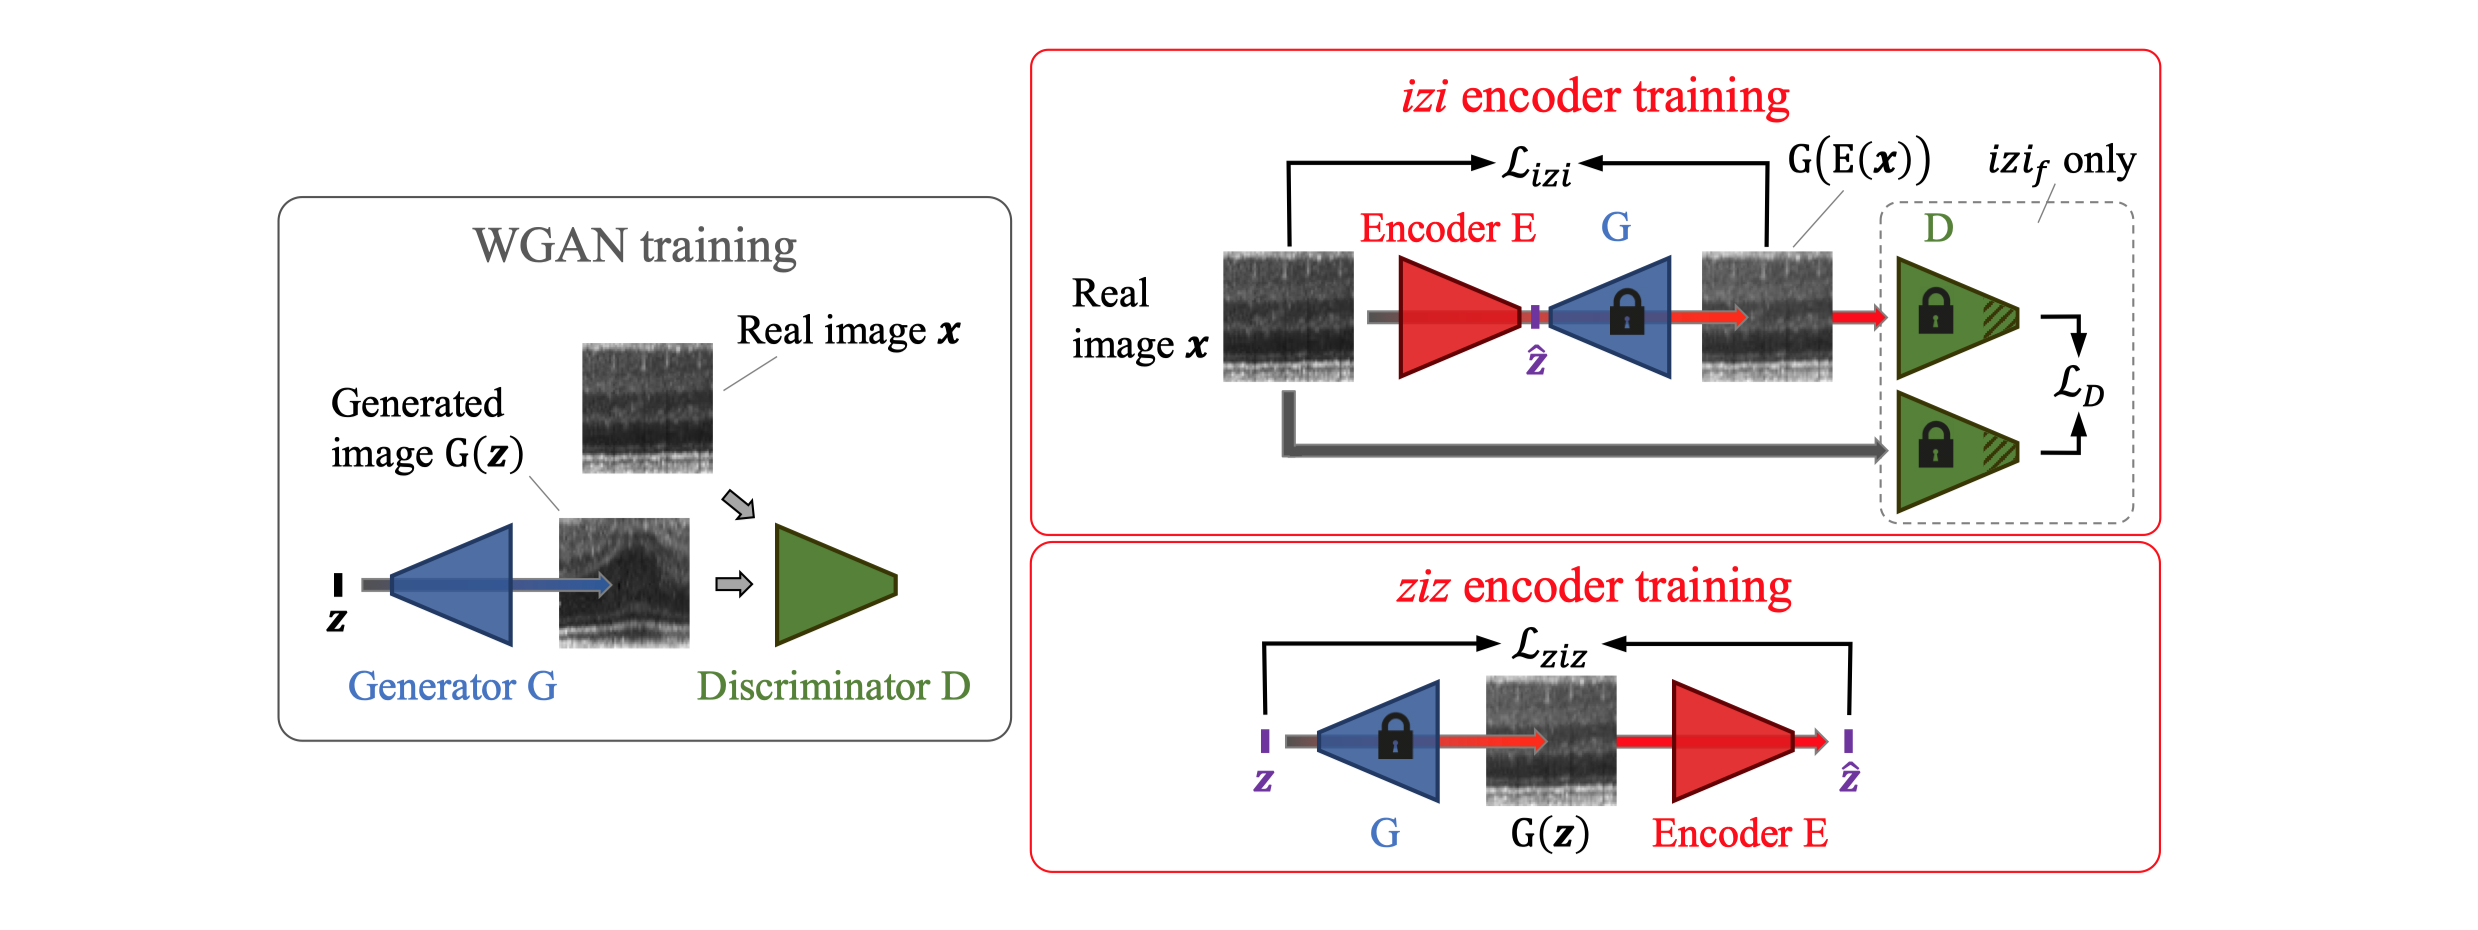
\includegraphics[width=.9\textwidth]{fanogan_training}
	\caption{F-AnoGAN Training Strategies \cite{pub.1111824956}}
	\label{fig:fanogan_training}
\end{figure}

This new training scheme comprises of two stages. In the first stage GAN model is trained.
Objective function for the adversarial training is also replaced with the Wasserstein GAN's
objective function \cite{Arjovsky2017WassersteinG} 
% appendix explanation ?
although training of the GAN can be performed with other training methods (including the
original GAN) according to the \cite{pub.1111824956}.

In the second stage, encoder network is trained using generator and discriminator networks with fixed
weights. Two separate pipelines are used to measure the performance of the encoder network. These are $IZI$
(image-noise-image) and $ZIZ$ (noise-image-noise) respectively. 

\textbf{IZI Encoder Training}

$IZI$ method follows the standard autoencoder network architecture. Generator network with fixed
weights acts as a decoder network. During the training, same image dataset used in the first stage
for training GAN is mapped to a latent space $z$ by a trainable encoder and then reconstructed
using the fixed generator network. Training objective for this setup is to minimize MSE (Mean
Squared Error) based reconstruction error of the input image $x$ and the reconstructed image
$G(E(x))$. 
\begin{equation}
	\mathcal{L}_{i z i}(\mathbf{x})=\frac{1}{n}\|\mathbf{x}-G(E(\mathbf{x}))\|^{2}
\end{equation}
where $n$ is the total dimension size of the data.
This approach has an important drawback regarding to latent representation. Since the distribution
of the latent representation of the input image is not known, the encoder is trained only using a
form of contextual loss which enforce the similarity only in the image space. Without the
sufficient information about the latent space, encoder may map images to a representations such
that the reconstructions are not convincing enough for the discriminator to evaluate as real
\cite{pub.1111824956}. Therefore model suggests including a latent space based loss
function derived from the feature layer of the discriminator network to guide the encoder network 
training. Improved $IZI_{f}$ training objective is defined below.
\begin{equation}
	\mathcal{L}_{i z i_{f}}(\mathbf{x})=\frac{1}{n} \cdot\|\mathbf{x}-G(E(\mathbf{x}))\|^{2}+\frac{\kappa}{n_{d}} \cdot\|f(\mathbf{x})-f(G(E(\mathbf{x})))\|^{2}
\end{equation}

where the $f(\cdot)$ represents the feature layer of the discriminator as an additional statistics, $n_{d}$ is
the dimensionality of the intermediate feature representation $f$ and $\kappa$ denotes the weighting
factor for the inclusion of the discriminator guidance.

\textbf{ZIZ Encoder Training}

This method reverses pipeline created on $IZI$ training and forms a decoder
encoder architecture. A random sampled noise from the latent $z$ space is mapped to the image space using the
fixed generator and then generated sample is encoded using the trainable encoder network. Loss
for the training objective is defined as the MSE based reconstruction of the noise which depicted in Equation
\ref{eqn:ziz} where $d$ is the total dimension of the latent representation.
\begin{equation}
\label{eqn:ziz}
	\mathcal{L}_{z i z}(\mathbf{z})=\frac{1}{d}\|\mathbf{z}-E(G(\mathbf{z}))\|^{2}
\end{equation}

Main shortcoming of this approach is that even though the encoder network is trained with a loss that will
enforce a similarity in latent space, encoder sees only images that are generated by the generator network.
It doesn't see any image samples from the training dataset which affects the contextual similarity
of the reconstruction of learned latent space distribution. 

\begin{figure}[h!] 
	\subfloat[Anomaly Score computation scheme for izi and $izi_f$ method]{
		\begin{minipage}[c][0.5\width]{0.5\textwidth}
			\centering
			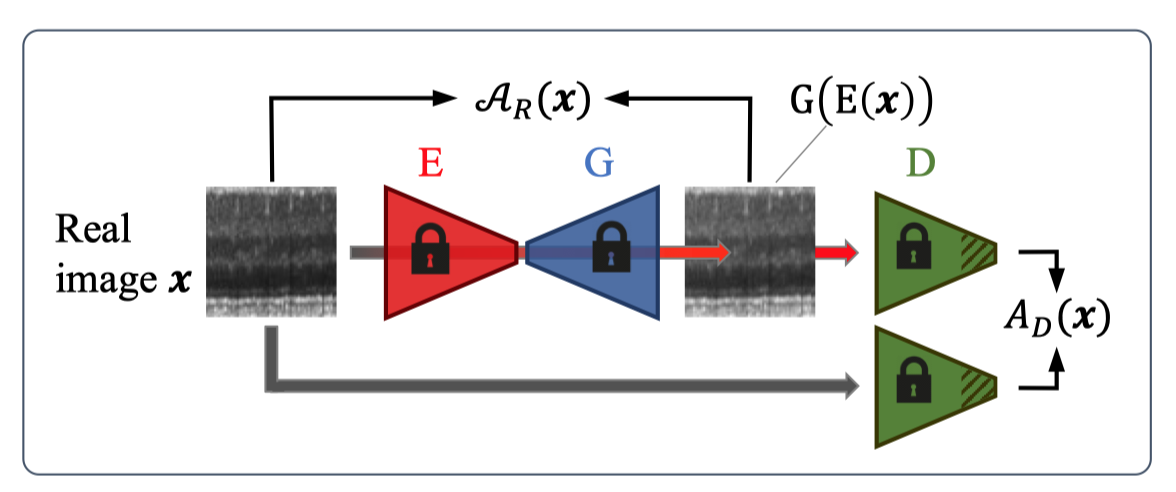
\includegraphics[width=1\textwidth]{fanogan_anomaly_1}
	\end{minipage}}
	\hspace*{\fill}%
	\subfloat[Anomaly Score computation scheme for ziz architecture]{
		\begin{minipage}[c][0.5\width]{0.5\textwidth}
			\centering
			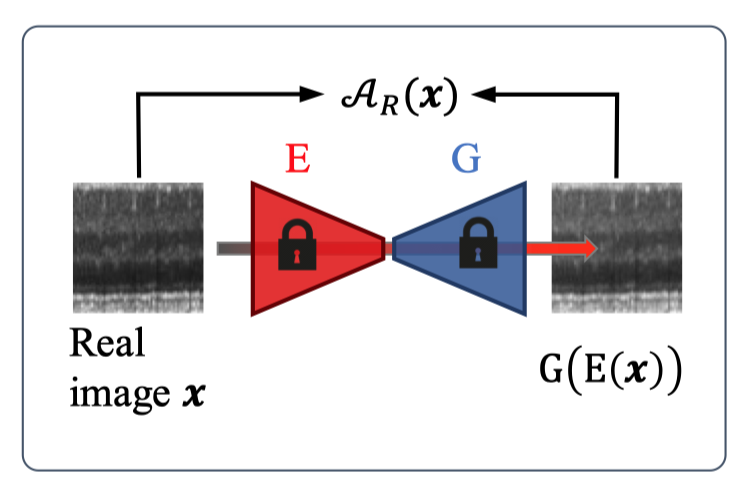
\includegraphics[width=0.6\textwidth]{fanogan_anomaly_2}
	\end{minipage}}
	\caption{Anomaly Score computations for both training methods \cite{pub.1111824956}}
	\label{fig:fanogan_anomaly_score}
\end{figure}

To calculate the anomaly score for inference, deviation of the query images from their
reconstructions are quantified. Figure \ref{fig:fanogan_anomaly_score} represents the anomaly score
computations for both training methods.

 $IZI_f$ method uses the same loss functions for the computation of the anomaly score. Anomaly score
 for image $x$ is defined as:
\begin{align}
	\mathcal{A}(\mathbf{x})&=\mathcal{A}_{R}(\mathbf{x})+\kappa \cdot \mathcal{A}_{D}(\mathbf{x}) \\[5pt]
	\mathcal{A}_{R}(\mathbf{x})&=\frac{1}{n} \cdot\|\mathbf{x}-G(E(\mathbf{x}))\|^{2} \\[5pt]
	\mathcal{A}_{D}(\mathbf{x})&=\frac{1}{n_{d}} \cdot\|f(\mathbf{x})-f(G(E(\mathbf{x})))\|^{2}
\end{align}

where $\mathcal{A}_R (x)$ represents the reconstruction based loss and $\mathcal{A}_{D} (x)$ represents the 
latent loss that uses feature layer of discriminator network.
For $IZI$ and $ZIZ$ method, the computation of the anomaly score reduces down to
$\mathcal{A}_{R}(\mathbf{x})$ function only. Both training methods yields a similar anomaly score
computation for the anomalous samples. Since the models are trained with a dataset that doesn't
contain any anomalies, query images that have anomalous regions results in poorer reconstruction
hence a higher anomaly score while the normal images produce a more similar reconstructions to the
original sample.
 
Significance of this model is that it separates the training of encoder network from the
adversarial setting of the GAN's while preserving the inverse mapping functionality for the
inference and keeping the inference time of the model relatively short. Chapter 
\ref{chap:arim} will explain its contribution to the proposed model.

} %%%%%%%%% CONTROL POINT
%%%%%%%%%%%%%%%%%%%%%%%%%%
\section{Energy Based Generative Adversarial Networks}
\label{sec:ebgan}

Training a GAN perhaps the most sensitive part of working with them. There has been an
extensive amount of research to improve the stabilization of the adversarial training or perhaps
offer a new methodology. \cite{fm} and \cite{methods} offer number modifications to the original
adversarial training setup to improve the generation performance ,increase the stabilization and
prevent issues such as mode collapse\footnotemark. \cite{Arjovsky2017WassersteinG} and
\cite{Gulrajani2017ImprovedTO} offers a new method to compute the loss and ways to stabilize it.
Mainly because of its adversarial setting, training of GANs will always be a topic of
interest. Energy based generative adversarial networks \cite{Zhao2016EnergybasedGA} offers a new
training method by redefining the loss functions and the functionality of the discriminator network.
This section will introduce the architecture and how it works.

\footnotetext{Mode collapse is the scenerio where generator learns enough information to fool the 
	discriminator very early. It finds a generation that fools the discriminator and does not learn 
	anything else from the discriminator. Because of that all the generated samples from the generator 
	look the same, defeating the purpose of generating from the distribution of the data.\cite{methods}}

Energy based models measures the current state of the model by assigning a scalar predefined energy
as a degree of compatibility \cite{LeCun06atutorial}. Training energy based models consists of
mapping low energy outputs to the samples with the "correct" class, and mapping higher energy
outputs to the "incorrect" class. From the perspective of GANs, EBGAN model is trained to ouput
lower energy for the real data, while the generated data (fake images) outputs a higher energy. The
model architecture can be seen in figure \ref{fig:ebgan_model}.

\begin{figure}[h!]
	\centering
	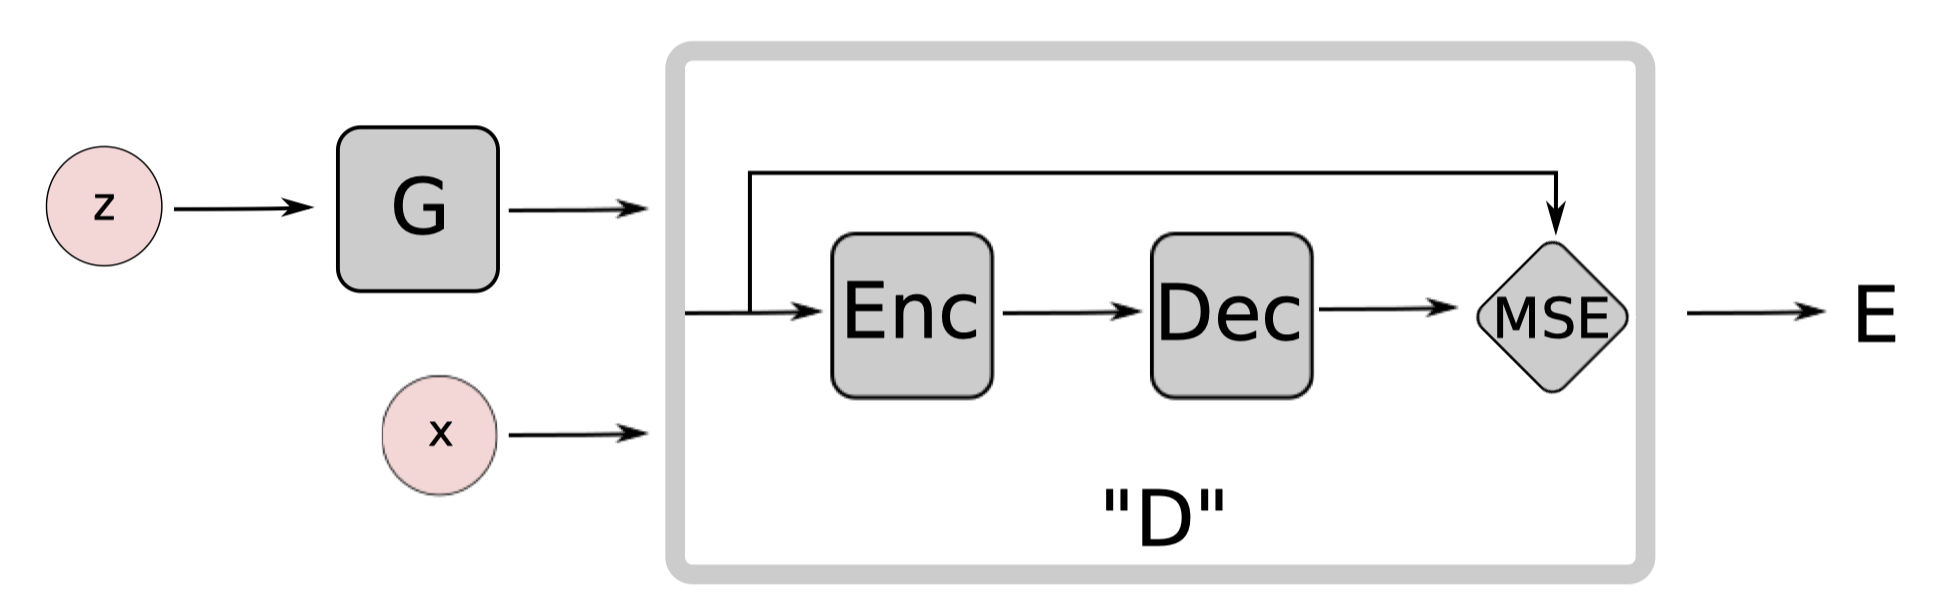
\includegraphics[width=1.0\textwidth]{ebgan_model}
	\caption{EBGAN Model Structure \cite{Zhao2016EnergybasedGA}}
	\label{fig:ebgan_model}
\end{figure}

The main structural difference of this framework from the other ones is that discriminator is
defined as an auto encoder network to provide the reconstruction of the inputs. The energy value
function is defined as the margin loss of the input and the reconstructed sample
\cite{Zhao2016EnergybasedGA} as a reconstruction error. 

Formally a margin is used to create an energy gap between the correct output and the incorrect
output. For data sample $x$, and a generated sample $G(z)$ with $z$ being sampled from a known
distribution $p_z$, The discriminator loss $\mathcal{L}_{D}$ and the generator loss
$\mathcal{L}_{G}$ are formally defined in equation \ref{eqn:ebgan_formal}.

\begin{equation}
\label{eqn:ebgan_formal}
\begin{aligned}D(x)&=\|\operatorname{Dec}(E n c(x))-x\|\\ \mathcal{L}_{D}(x, z) &=D(x)+[m-D(G(z))]^{+} \\ \mathcal{L}_{G}(z) &=D(G(z)) \end{aligned}
\end{equation}

where $D(x)$ is the reconstuction loss and  $[\cdot]^{+}=\max (0, \cdot)$. Minimizing
$\mathcal{L}_{G}$ with respect to the generator is similar to maximizing the second term of the
$\mathcal{L}_{D}$. Instead of calculating the probability of the input being real or fake,
discriminator is responsible for attaining the correct amount of energy to the input images. 

Using autoencoder network as a discriminator brings additional advantages to the training setting.
Rather than using a single target information to train the model, reconstruction based output offers
a more diverse targets for the discriminator \cite{Zhao2016EnergybasedGA}. One of the reasons that causes
stabilization issues in the adversarial training is that discriminator might provide gradients not
useful enough for generator to improve the quality of the generated samples. Having a reconstruction
loss output might provide a better gradient in terms of different directions as opposed to binary
logistic loss\cite{Zhao2016EnergybasedGA}. Another advantage is that even though they are trained with an adversarial setting,
autoencoder networks might prove useful to learn the underlying energy manifold of the data without
supervision or negative examples when they are trained using a proper regularization constraint.
This means that in this setting generated samples and input data are both used to model the
underlying energy manifold of the data. 

EBGAN argues that, the discriminator network is regularized by exposing generated samples
from the generator  which it should output higher reconstruction energies
\cite{Zhao2016EnergybasedGA}. The benefit of this regularization is that instead of a hand crafted
predefined one, the regularization term can also be trained along with the discriminator.
Adversarial training allows a direct connection between learning the energy function and producing
contradictive samples in that regard. 

EBGAN also adds additional penalty called pulling away term (PT) that run at a
representation level to prevent mode collapse depicted in equation \ref{eqn:ebgan_pt}.
\begin{equation}
\label{eqn:ebgan_pt}
	f_{P T}(S)=\frac{1}{N(N-1)} \sum_{i} \sum_{j \neq i}\left(\frac{S_{i}^{\top} S_{j}}{\left\|S_{i}\right\|\left\|S_{j}\right\|}\right)^{2}
\end{equation}

 $S$ is the feature output from the encoder for generated images. Pulling-away term measures the
 cosine similarity among all generated images features $S$ in a minibatch. If the mode collapses,
 the feature vectors will thereupon be similar, i.e. the angles are close to zero and the cosine
 will max-out. Therefore, it will add a high penalty if there are too similar.
 \cite{Zhao2016EnergybasedGA}
 
 EBGAN offers a more flexible approach to train the discriminator and generator network. 
 Transition from convolutional based discriminator to autoencoder network also provides a potential inclusion 
 for the computation of the anomaly score. Its impact on the proposed model will be discussed in the next chapter. 

\endgroup
